\begin{figure}[H]
	\centering
	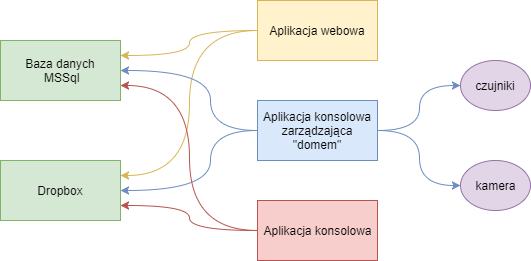
\includegraphics[scale=0.8]{schemat_systemu.png}
	\caption{Budowa systemu zarządzania domem}
	\label{fig:schemat_systemu}
\end{figure}
Aplikację powstałą na potrzeby tej pracy można podzielić na 3 moduły, które zostały przedstawione na rysunku \ref{fig:schemat_systemu}, a składają się na nie :
\begin{itemize}
\item Aplikacja webowa- interfejs pozwalający na zlecanie nowych zadań aplikacji konsolowej oraz odczyt wyników przesłanych przez nią oraz przez program zarządzający domem,
\item Aplikacja konsolowa- przetwarza zadania detekcji oraz rozpoznawania twarzy zlecone za pomocą aplikacji webowej,
\item Program zarządzający domem- przekazuje cyklicznie odczytywane dane z czujników oraz wykryte ruchy do bazy danych, w celu dalszej obróbki przez pozostałe moduły.
\end{itemize}
Na usługi pomocnicze wykorzystane w projekcie składają się
\begin{itemize}
\item baza danych- przechowywanie danych o dodanych zadaniach, wynikach, nauczonych sieciach neuronowych oraz osobach,
\item dropbox- przechowywanie większych plików- obrazów oraz nauczonych modeli sieci.
\end{itemize}

\section{Aplikacja webowa}
Aplikacja webowa jest jedyną częścią systemu, do której użytkownik może mieć bezpośredni dostęp. Strona powstała w celu maksymalnego uproszczenia procesu badania kolejnych algorytmów i usług, które różniły się sposobem podawania danych wejściowych, sposobem uczenia oraz formatem zwracanych odpowiedzi. Do pozostałych zalet takiego rozwiązania należy ułatwienie przechowywania danych, poprzez umieszczenie ich we wspólnym miejscu co pomaga, w późniejszej interpretacji wyników.
\begin{figure}[H]
	\centering
	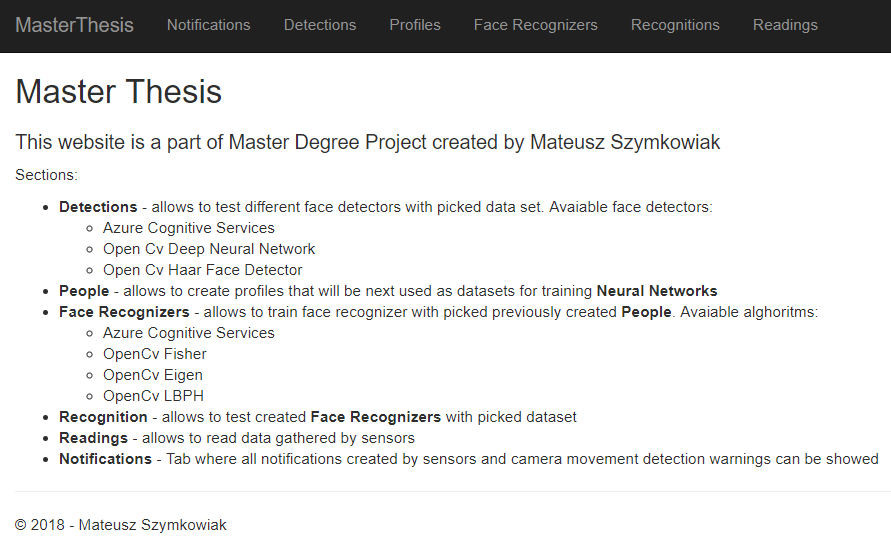
\includegraphics[scale=0.7]{aplikacja_webowa_razor_widok.png}
	\caption{Wygląd strony głównej}
	\label{fig:strona_glowna_razor}
\end{figure}
Zgodnie z interfejsem przedstawionym na rysunku \ref{fig:strona_glowna_razor}, strona została podzielona na 5 głównych sekcji:
\begin{itemize}
\item Detections- detekcje,
\item People- ludzie,
\item Neural Networks- sieci neuronowe,
\item Recognition- rozpoznawanie,
\item Sensor Readings- odczyty sensorów.
\end{itemize}

\subsection{Technologie}
Aplikacja webowa powstała w najnowszej kompilacji .NET Core 2, będącej międzyplatformową strukturą open source o wysokiej wydajności służącą do tworzenia nowoczesnych aplikacji internetowych opartych na usługach chmurowych. Logika biznesowa aplikacji została zaprogramowana w języku C\#. Warstwa widoku powstała w dwóch dostępnych rozwiązaniach, nieznacznie różniących się wyglądem, ale znacznie odbiegających od siebie sposobem działania. Przed omówieniem poszczególnych rozwiązań przedstawiono, krótkie definicje wykorzystanego wzorca projektowego MVC oraz technologii SPA

\subsubsection{Wzorzec projektowy MVC}
\begin{figure}[H]
	\centering
	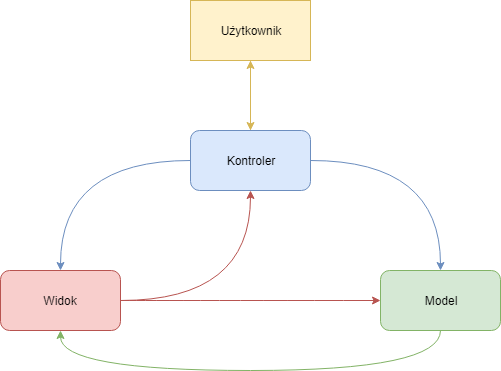
\includegraphics[scale=0.8]{mvc.png}
	\caption{Schemat klasycznego wzorca MVC}
	\label{fig:schemat_mvc}
\end{figure}
Strona internetowa powstała na bazie bardzo popularnego wśród programistów wzorca projektowego MVC. Założenia wzorca Model-Widok-Kontroler są bardzo proste, ich składowymi są:
\begin{itemize}
\item Model- reprezentuje logikę biznesową. Tutaj znajdują się wszelkie obiekty, które służą do wykonywania zaimplementowanej funkcjonalności danej aplikacji,
\item Widok- jest warstwą prezentacji. Odpowiada za prezentację logiki biznesowej (Modelu) użytkownikowi w przystępny sposób,
\item Kontroler- obsługuje żądania użytkownika. Odebrane zadania oddelegowuje do odpowiednich modeli.
\end{itemize}

\subsubsection{Single Page Application}
Single Page Application (SPA) to aplikacja lub strona internetowa, która w całości wczytuje się za jednym razem. Cały potrzebny do działania strony kod (HTML, CSS, JavaScript) przesyłany jest na początku lub dodawany dynamicznie w kawałkach, zwykle w odpowiedzi na interakcje generowane przez użytkownika.
Sposób działania takiej aplikacji jest zbliżony do odczuć towarzyszących korzystaniu z aplikacji desktopowej lub mobilnej. 

\subsubsection{Rozwiązanie 1- Razor Pages}
Pierwsza wersja została oparta o strony tworzone w technologi Razor Pages opartej o składnię Razor oraz podstawowe technologie webowe: HTML i CSS. Taki sposób tworzenia warstwy prezentacji jest zalecany dla aplikacji .NET Core, ponieważ pozwala zminimalizować ilość pracy wymaganej na jej utworzenie oraz zapewnia bardzo prosty proces wdrożenia. Aplikacja utworzona z pomocą Razor'a została zaprezentowana na rysunku \ref{fig:strona_glowna_razor}.

\subsubsection{Rozwiązanie 2- Angular 4}
Druga wersja widoku aplikacji oferuje dostęp do tych samych możliwości co pierwsze rozwiązanie, ale powstała przy pomocy frameworka webowego- Angular 4. Strona główna widoczna jest na rysunku \ref{fig:strona_glowna_angular}. Angular jest open sourcowym frameworkiem używanym do tworzenia aplikacji SPA (Single Page Application), napisany w języku TypeScript i wspierany oraz rozwijany przez Google.
\begin{figure}[H]
	\centering
	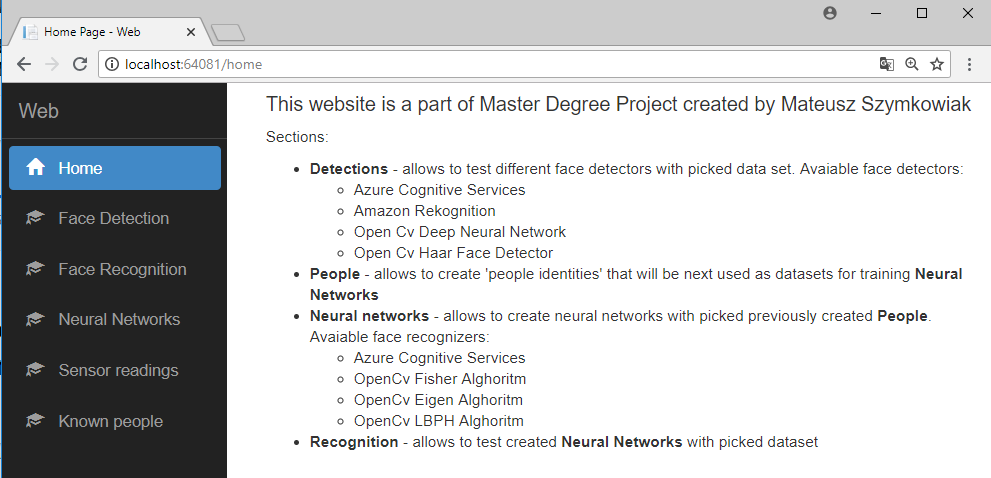
\includegraphics[scale=0.6]{aplikacja_webowa_angular_widok.png}
	\caption{Strona główna widoku utworzonym w Angular 4}
	\label{fig:strona_glowna_angular}
\end{figure}

\subsection{Detections}
Detections jest stroną odpowiedzialną za wykrywanie twarzy na obrazach przesłanych do systemu. Na głównej stronie możemy zobaczyć wszystkie zlecone detekcje, zarówno nowe jak i już zakończone.
\begin{figure}[H]
	\centering
	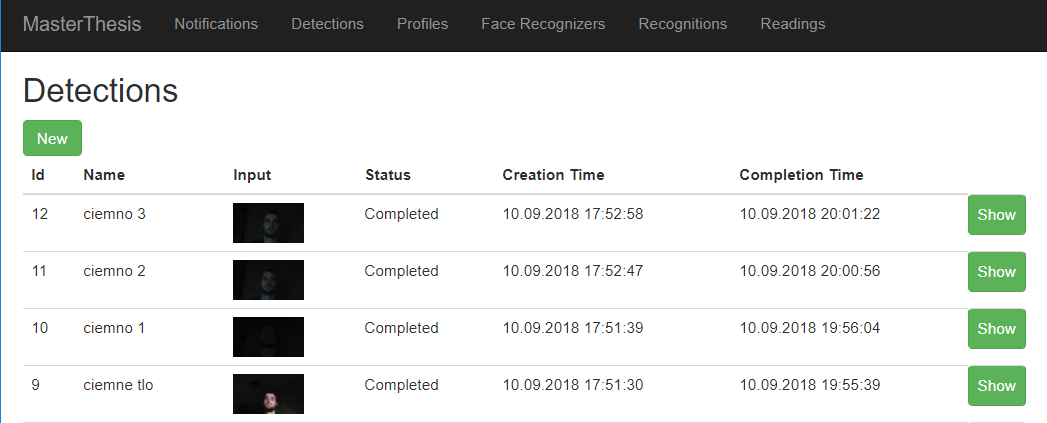
\includegraphics[scale=0.6]{detections.png}
	\caption{Widok detekcji twarzy}
	\label{fig:detections}
\end{figure}
Przycisk 'New' widoczny na \ref{fig:detections} pozwala na stworzenie nowego zadania wykrycia twarzy na obrazie, które zostanie przetworzone przez moduł aplikacji konsolowej. Na formularzu z rysunku \ref{fig:new_detection} należy podać nazwę zadania oraz za pomocą przycisku 'Wybierz plik' wybrać obraz w formacie png,jpg lub jpeg znajdujący się na dysku użytkownika.
\begin{figure}[H]
	\centering
	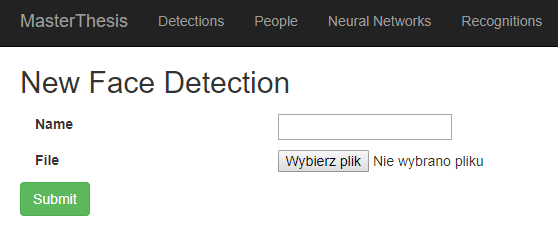
\includegraphics[scale=0.6]{new_detection.png}
	\caption{Tworzenie nowej detekcji}
	\label{fig:new_detection}
\end{figure}
Użycie przycisku 'Show' widocznego przy każdym zadaniu detekcji na rysunku \ref{fig:detections}, pozwoli na wyświetlenie szczegółów związanych z requestem, w tym wyników jeśli zadanie zostało zakończone.
\begin{figure}[H]
	\centering
	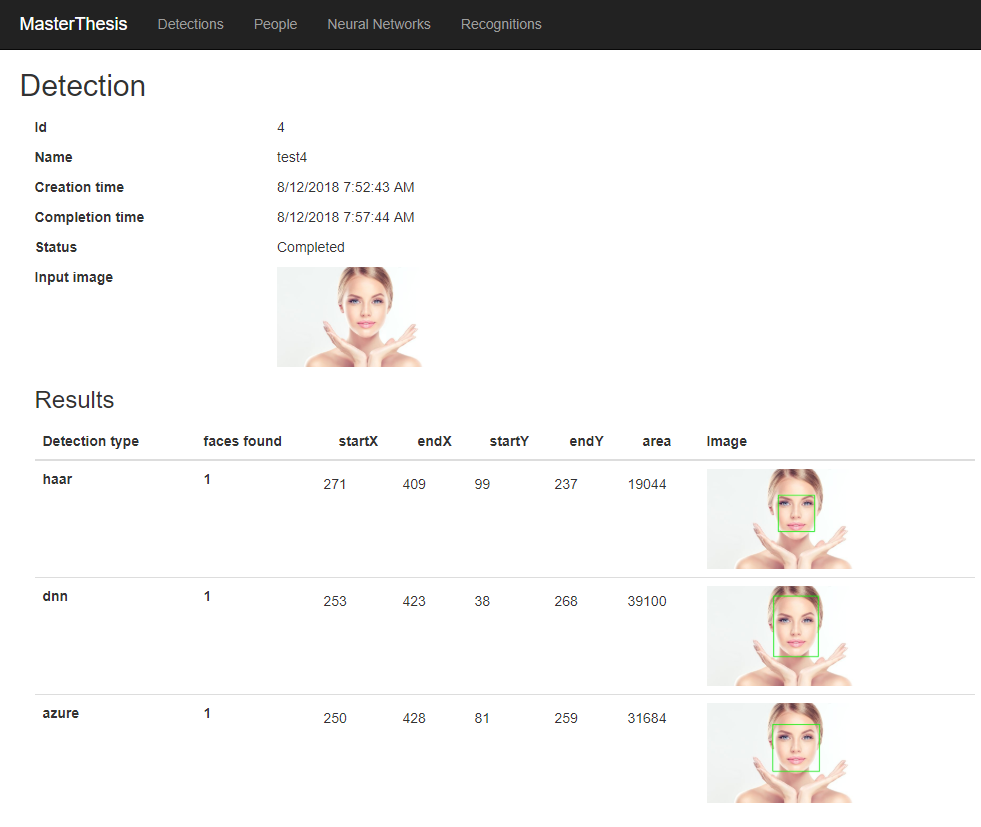
\includegraphics[scale=0.6]{detekcja_z_wynikami.png}
	\caption{Widok zakończonej detekcji}
	\label{fig:detekcja_zakonczona}
\end{figure}
Strona ze zdjęcia \ref{fig:detekcja_zakonczona} pozwala sprawdzić datę utworzenia oraz zakończenia zadania, obraz wejściowy, szczegółowe informacje o obszarze zidentyfikowanym jako twarz oraz sposobie jej wykrycia.
\subsection{People}
Strona 'People' służy do tworzenia nowych znanych tożsamości, które później mogą zostać wykorzystane jako dane uczące podczas trenowania sieci neuronowych. Do każdej osoby musi zostać przypisany zasób minimum 2 zdjęć. W przypadku braku możliwości wykrycia twarzy na zdjęciu, zostanie ono zignorowane podczas procesu nauczania.
\begin{figure}[H]
	\centering
	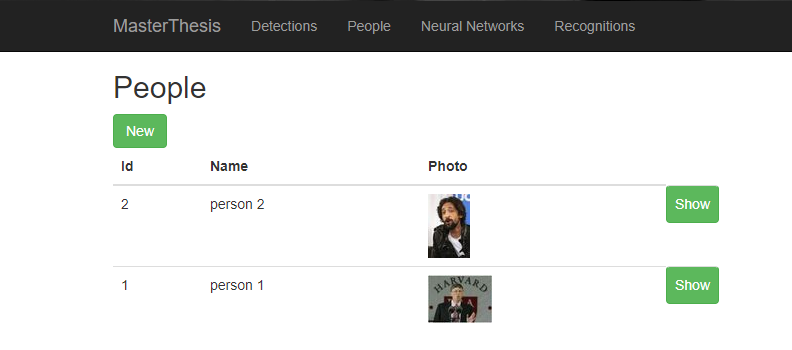
\includegraphics[scale=0.6]{people.png}
	\caption{Lista utworzonych ludzi}
	\label{fig:people}
\end{figure}
Nowa osoba może zostać utworzona w podobny sposób jak request detekcji twarzy. Jedyną różnicą jest wymóg wyboru kilku obrazów.
\begin{figure}[H]
	\centering
	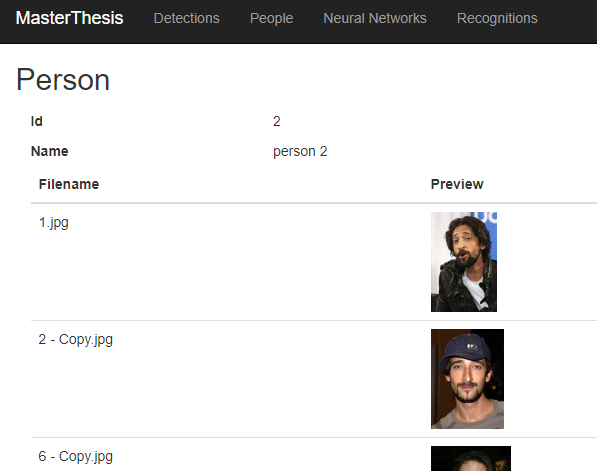
\includegraphics[scale=0.6]{person.png}
	\caption{Widok osoby}
	\label{fig:person}
\end{figure}
Utworzona osoba nie może być modyfikowana. Pierwsze załadowanie widoku osoby może trwać wydłużony czas z powodu procesu generowania linków do plików magazynowanych w usłudze Dropbox.

\subsection{Neural Networks}
\begin{figure}[H]
	\centering
	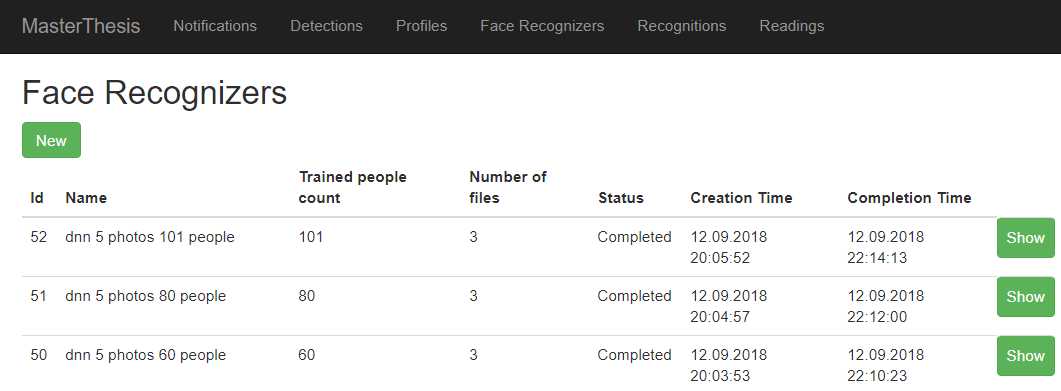
\includegraphics[scale=0.6]{neural_networks.png}
	\caption{Strona przedstawiająca istniejące grupy usług rozpoznawania tożsamości}
	\label{fig:sieci_neuronowe}
\end{figure}
W zakładce 'Neural Networks' użytkownik ma możliwość stworzenia grupy wybranych usług i sieci neuronowych, które zostaną nauczone rozpoznawać tożsamości utworzone w zakładce 'People'.
\begin{figure}[H]
	\centering
	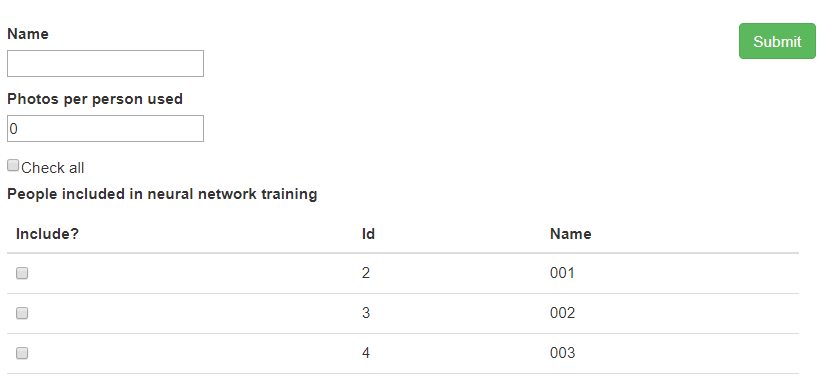
\includegraphics[scale=0.6]{nowa_siec.png}
	\caption{Tworzenie nowej grupy sieci neuronowych}
	\label{fig:nowa_siec}
\end{figure}
Każda istniejąca osoba zostanie wyświetlona jako checkbox, który należy zaznaczyć jeśli użytkownik chce by dana osoba została wykorzystana podczas procesu trenowania. Należy wybrać minimum 2 osoby, w przypadku wyboru mniejszej ilości osób, użytkownik zostanie poinformowany o tej konieczności.

Widok ukazany na rysunku \ref{fig:sieci_neuronowe} pozwala sprawdzić ile osób zostało użytych w procesie nauki oraz ile sieci neuronowych zostało utworzonych. Wyświetlenie jednej z grup pozwoli na uzyskanie bardziej szczegółowych informacji na temat wykorzystanych osób i utworzonych sieci, patrz rysunek \ref{fig:siec_neuronowa}.
\begin{figure}[H]
	\centering
	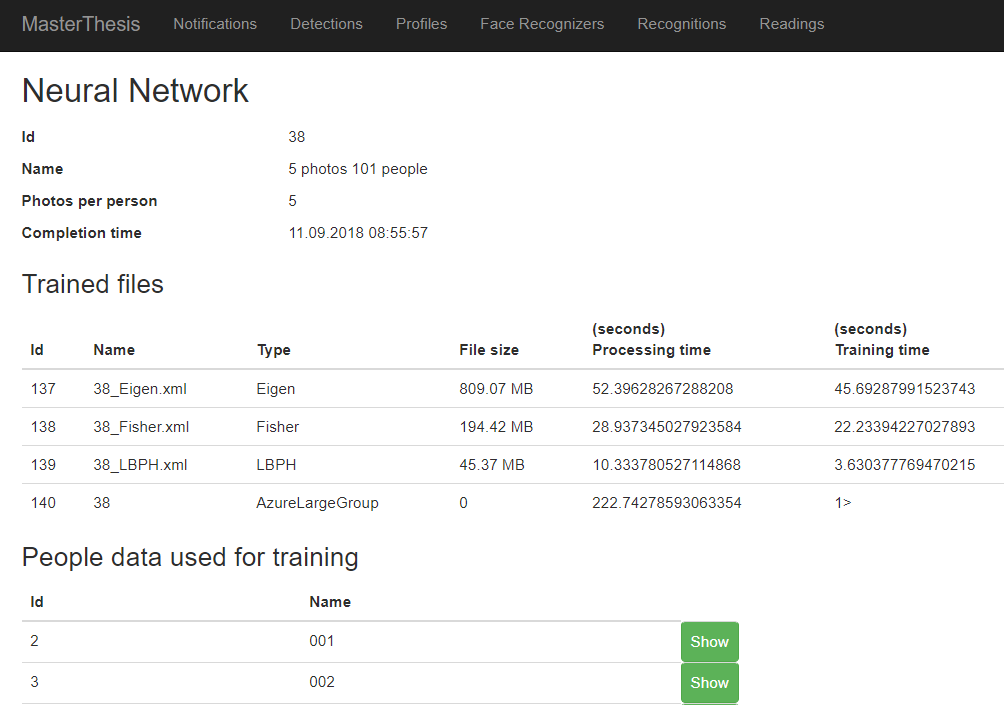
\includegraphics[scale=0.6]{siec_neuronowa.png}
	\caption{Szczegółowe informacje o grupie sieci neuronowych}
	\label{fig:siec_neuronowa}
\end{figure}

\subsection{Recognitions}

\section{Aplikacja konsolowa}

\section{Program zarządzający domem}